\documentclass[Serif, 10pt, brown]{beamer}
\usepackage{booktabs,xcolor}
\usepackage{pifont}
\newcommand*\CHECK{\ding{51}}
\usepackage{array}
\newcolumntype{P}[1]{>{\centering\arraybackslash}p{#1}}

\usepackage{setspace,mathtools,amssymb,multirow,array,amsmath,tikz}
\usepackage[normalsize]{subfigure}
\usetikzlibrary{patterns,automata,positioning,decorations.pathreplacing,decorations}
\usepackage{curves}
\usepackage{caption}
\usepackage{wasysym}
\usepackage{epsfig,epstopdf,graphicx}

\curvewarnfalse

\newtheorem{proposition}{Proposition}
\theoremstyle{example}
\newtheorem{theoremh}{Theorem}
\theoremstyle{plain}
\renewcommand{\textfraction}{0.01}
\renewcommand{\floatpagefraction}{0.99}
\newcommand{\ul}{\underline}
\newcounter{units}
\setbeamercovered{dynamic}
\newcommand{\FIGDIR}{../figures} 
\newcommand{\RESULTDIR}{../../results} 
\logo{\includegraphics[width=0.5in,keepaspectratio]{\FIGDIR/iitb_logo.png}}

\mode<presentation>{
    \usetheme[right,currentsection,hideothersubsections]{UTD}
    \useoutertheme{sidebar}
    \useinnertheme[shadow]{rounded}
    \usecolortheme{whale}
    \usecolortheme{orchid}
    \usefonttheme[onlymath]{serif}
    \setbeamertemplate{footline}{\centerline{Slide \insertframenumber/\inserttotalframenumber}}
}

\usebeamercolor[fg]{author in sidebar}
\title[{Systems for LLMs}]{\sc Profiling and Optimizing LLM Inference at Scale}
\author[\ul{Saksham Rathi}]{{\textbf{Saksham Rathi}}}
\institute[UTD]{\sc\small Bachelor's Thesis Project - Stage 1\\ Under Prof. Mythili Vutukuru}
\date[UCI]{Indian Institute of Technology Bombay \\ Autumn 2025-26}

\begin{document}
\frame{\titlepage}

\begin{frame}{Contents}
	\tableofcontents
\end{frame}

\section{Introduction}
\begin{frame}{Motivation}
    \begin{itemize}
        \item In many real-world settings, multiple users query the same underlying document or system prompt. \pause
        \item For example, an Operating Systems teaching assistant bot may maintain a large shared context of lecture notes and examples, while each student asks short, context-specific questions. \pause
        \item Similarly, enterprise assistants handle hundreds of independent queries over a shared knowledge base or product documentation. \pause
        \item Recomputing attention over identical prefixes leads to redundant computation and wasted GPU cycles. \pause
        \item Additionally, memory usage grows rapidly with batch size and KV cache accumulation.
    \end{itemize}
\end{frame}

\begin{frame}{Problem Statement}
    \begin{itemize}
        \item Our goal is to characterize and analyze the performance of LLM inference workloads with shared prefixes. \pause
        \item What are the key GPU-level metrics for evaluating such workloads? \pause
        \item How do modern inference engines optimize for shared-prefix execution? \pause
        \item How do mechanisms like prefix caching, chunked prefill, and request scheduling impact throughput and latency? \pause
        \item What bottlenecks limit scalability as the number of concurrent prefix families increases?
    \end{itemize}
\end{frame}

\section{Background}

\begin{frame}{Prefill vs Decode}
\begin{itemize}
    \item \textbf{Prefill:} Takes the whole user prompt as input and computes the probability of the first new token. Generate key and value vectors. Can be parallelized because all the tokens are known. \pause
    \item \textbf{Decode:} Generates the remaining new tokens sequentially. Stops when the maximum length is reached, or when an end-of-sequence token is emitted. Autoregressive in nature.
\end{itemize}
\end{frame}

\begin{frame}{Inference Engines}
    \begin{columns}[T, totalwidth=\textwidth]
        \begin{column}{0.4\textwidth}
            \centering
            \includegraphics[width=\textwidth]{\FIGDIR/arch.png}
            \vspace{0.3em}
            \captionof{figure}{Architecture of a LLM}
            \centering
            \includegraphics[width=\textwidth]{\FIGDIR/llm-inference-n-serving.drawio.png.png}
            \vspace{0.3em}
            \captionof{figure}{Architecture of an Inference Engine}
        \end{column}
        \begin{column}{0.6\textwidth}
            \begin{itemize}
                \item Systems layer that manages the execution of large language model (LLM) inference on hardware resources. \pause
                \item Multiple user requests are grouped into a single batch to maximize GPU utilization and reduce per-request overhead. \pause
                \item Memory Storage: Cache key-value pairs, reuse memory buffers, and apply quantization or weight-sharing. \pause
                \item Offloading: Portions of the model state or intermediate activations can be offloaded to CPU when not needed actively.
            \end{itemize}
        \end{column}
    \end{columns}
\end{frame}



\section{Prior Work}

\begin{frame}{vLLM}
    \begin{itemize}
        \item vLLM adopts a centralized scheduler to coordinate the execution of distributed GPU workers. \pause
        \item PagedAttention partitions the KV cache of each sequence into KV blocks. Removes internal and external fragmentation. \pause
        \item Allows blocks to be shared when multiple samples share the same input prompt, or during beam search. Implements copy-on-write mechanism at the block granularity for the physical blocks that need modification by multiple sequences. \pause
        \item Evicted blocks are copied to the CPU memory.  \pause
        \item Each cached block is identified by the block hash - which comprises of the parent block hash, block tokens, and some extra fields.
    \end{itemize}
\end{frame}

\begin{frame}{FastTree}
    \begin{columns}[T, totalwidth=\textwidth]
        \begin{column}{0.4\textwidth}
            \centering
            \includegraphics[width=\textwidth]{\FIGDIR/kv_cache_sharing_through_radix_tree.png}
            \vspace{0.3em}
            \captionof{figure}{KV Cache Sharing through RadixTree}
        \end{column}
        \begin{column}{0.6\textwidth}
            \begin{itemize}
                \item Introduces GPU kernels specifically designed to process queries that share common prefixes within a radix tree structure. \pause
                \item Gives an optimal edge assignment based on two types of losses - (1) Tile Padding (2) Maintaining Intermediate results \pause
                \item Merges queries with the same prefix into a single kernel - (1) Decreases global memory transactions (2) Converts GEMV to GEMM operations
            \end{itemize}
        \end{column}
    \end{columns}
\end{frame}

\section{Experiments - Single Family}
\begin{frame}{Workload Setup}
\begin{itemize}
    \item \textbf{Goal:} Evaluate inference performance of LLMs under short queries with large shared context. \pause
    \item \textbf{Models:} Qwen 0.5B, Tiny Llama 1.1B, Llama 3.1 8B, served using vLLM/SGLang/Transformers. \pause
    \item \textbf{Hardware:} NVIDIA RTX6000 48GB GPU. \pause
    \item \textbf{Metrics:} Throughput (req/s), latency, GPU utilization.
\end{itemize}

\begin{table}[h!]
\centering
\scriptsize
\begin{tabular}{|l|c|}
\hline
\textbf{Parameter} & \textbf{Value/Range} \\
\hline
System Prompt Length & $\approx$1500 tokens (shared across requests) \\
Query Rate & 5–700 req/sec \\
Query Length & 10–20 tokens \\
Output Length & 30–50 tokens \\
Batch Size & Adaptive \\
\hline
\end{tabular}
\caption{Workload Characteristics}
\end{table}
\end{frame}

\begin{frame}{Experiment Setup: Engine Comparison}
\begin{itemize}
    \item Compare inference engines: \textbf{Transformers}, \textbf{vLLM}, \textbf{SGLang}. \pause
    \item Batch of 24 requests, each sharing the same system prompt. \pause
    \item Each request: $\sim$20 input tokens $\rightarrow$ $\sim$40 generated tokens. \pause
    \item Measure \textbf{total time taken} to process the batch. \pause
\end{itemize}

\begin{block}{Hypothesis}
Engines leveraging prefix caching (e.g., SGLang) should perform far better than naive batching in Transformers.
\end{block}
\end{frame}

\begin{frame}{Batch of requests through various Engines}
    \begin{columns}[T, totalwidth=\textwidth]
        \begin{column}{0.4\textwidth}
            \centering
            \includegraphics[width=\textwidth]{\RESULTDIR/throughput_vs_qps.png}
            \vspace{0.3em}
            \captionof{figure}{Throughput comparison across varying workloads}
        \end{column}
        \begin{column}{0.6\textwidth}
            \begin{itemize}
                \item \textbf{SwiftLLM:} lightweight vLLM clone ($\sim$2000 LOC), but doesn't performs that well.
                \item \textbf{SGLang:} achieves best performance via radix-tree prefix sharing.
            \end{itemize}
            \begin{table}[h]
            \centering
            \scriptsize
            \begin{tabular}{|l|c|}
            \hline
            \textbf{Technique Used} & \textbf{Time (s)} \\
            \hline
            Transformers (batch = 1) & 30.21 \\
            Transformers (batch = 2) & 19.51 \\
            Transformers (batch = 3) & 18.64 \\
            vLLM (no system prompt pre-filling) & 0.45 \\
            SGLang (fork) & 1.03 \\
            SGLang (run\_batch) & 0.40 \\
            \hline
            \end{tabular}
            \caption{Measuring the time taken to process a batch of 24 requests using different techniques}
            \end{table}
        \end{column}
    \end{columns}
\end{frame}


\begin{frame}{Experiment Setup: Request Timelines}
\begin{itemize}
    \item Aim: Measure time spent in \textbf{prefill} vs \textbf{decode} stages for 20 req/sec workload (sending a new request after every 0.05 seconds). \pause
    \item Using vLLM V0 engine without chunked prefill. \pause
    \item Tool: Custom logging of per-request timestamps.
\end{itemize}
\begin{figure}[h!]
\centering
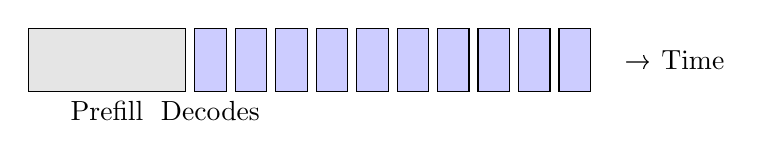
\begin{tikzpicture}[node distance=0.1cm]
\tikzstyle{block}=[draw,fill=gray!20,minimum height=0.8cm]
\def\prefillwidth{2cm}
\def\decodewidth{0.4cm}
\node[block,minimum width=\prefillwidth,label=below:{Prefill}] (p) {};

\foreach \i in {1,...,10} {
  \pgfmathtruncatemacro{\prev}{\i - 1}
  \ifnum\i=1
    \node[block,fill=blue!20,minimum width=\decodewidth,
          right=of p,label=below:{Decodes}] (d\i) {};
  \else
    \node[block,fill=blue!20,minimum width=\decodewidth,
          right=of d\prev,label=below:{}] (d\i) {};
  \fi
}
\node[right=of d10,xshift=0.2cm] {→ Time};

\end{tikzpicture}
\caption{Simplified per-request timeline}
\end{figure}
\end{frame}

\begin{frame}{Results: LLM Request Timelines}
\begin{columns}[T, totalwidth=\textwidth]
    \begin{column}{0.6\textwidth}
        \centering
        \includegraphics[width=\textwidth]{\FIGDIR/llm_timelines_20.png}
        \captionof{figure}{20 Requests/sec – No chunked prefill – vLLM V0}
    \end{column}
    \begin{column}{0.4\textwidth}
        \begin{itemize}
            \item Prefill dominates runtime due to large prompt. \pause
            \item Prefill and decode cannot overlap here. \pause
            \item Low TTFT but high total latency.
        \end{itemize}
    \end{column}
\end{columns}
\end{frame}

\begin{frame}{Results: Throughput vs Load for vLLM}
\begin{columns}[T, totalwidth=\textwidth]
    \begin{column}{0.6\textwidth}
        \centering
        \includegraphics[width=\textwidth]{\RESULTDIR/throughput_comparison_vllm.png}
        \captionof{figure}{Throughput vs Load}
    \end{column}
    \begin{column}{0.4\textwidth}
        \begin{itemize}
            \item Varying the input load, and comparing different modes. \pause
            \item Chunked prefill: limited benefit for small queries. \pause
            \item Prefix caching: major boost to throughput. \pause
            \item Batch tuning further improves efficiency. \pause
        \end{itemize}
    \end{column}
\end{columns}
\begin{block}{Observation}
    Saturation begins at $\sim$300 req/sec — compute bottleneck.
\end{block}
\end{frame}

\section{Metrics}
\begin{frame}{Key GPU Metrics}
    \begin{itemize}
        \item We employ two primary NVIDIA tools for this study: Nsight Systems (\textbf{NSYS}) and the Data Center GPU Management Interface (\textbf{DCGMI}). \pause
        \item \textbf{SM Activity:} The fraction of time at least one warp was active on a multiprocessor, averaged over all multiprocessors. \pause
        \item \textbf{SM Occupancy:} The fraction of resident warps on a multiprocessor, relative to the maximum number of concurrent warps supported on a multiprocessor. \pause
        \item \textbf{Tensor Core Utilization:} The fraction of cycles the tensor pipe was active.
    \end{itemize}
\end{frame}

\begin{frame}{NSYS Run on Matrix Multiplication}
    \begin{itemize}
        \item Various Phases: Host to device copy, kernel computation, and device to host copy.
        \item Compute metrics reach high values during kernel execution phase.
    \end{itemize}
\centering
\includegraphics[width=0.8\textwidth]{\FIGDIR/nsys_matmul.png}
\captionof{figure}{NSYS Metrics Snapshot}
\end{frame}


\section{Experiments - Multiple Families}

\begin{frame}{Multiple Families - Generation of such a workload}
    

\begin{figure}[h!]
\centering
\resizebox{0.9\textwidth}{!}{
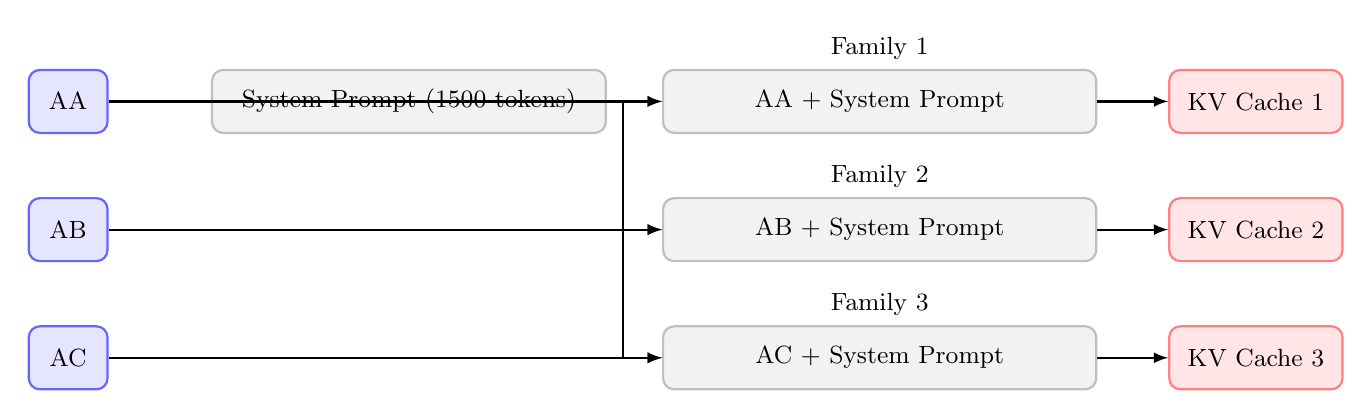
\begin{tikzpicture}[
    family/.style={rectangle, draw=blue!60, fill=blue!10, thick, rounded corners, minimum height=0.8cm, align=center},
    token/.style={rectangle, draw=gray!50, fill=gray!10, thick, rounded corners, minimum height=0.8cm, align=center},
    cache/.style={rectangle, draw=red!50, fill=red!10, thick, rounded corners, minimum height=0.8cm, align=center},
    arrow/.style={->, thick, >=latex},
    font=\small
]

\node[token, minimum width=5cm] (sys) {System Prompt (1500 tokens)};
\node[family, left=1.3cm of sys, minimum width=1cm] (aa) {AA};
\node[family, below=0.8cm of aa, minimum width=1cm] (ab) {AB};
\node[family, below=0.8cm of ab, minimum width=1cm] (ac) {AC};

\node[token, right=0.7cm of sys, minimum width=5.5cm, label=above:{Family 1}] (f1) {AA + System Prompt};
\node[token, below=0.8cm of f1, minimum width=5.5cm, label=above:{Family 2}] (f2) {AB + System Prompt};
\node[token, below=0.8cm of f2, minimum width=5.5cm, label=above:{Family 3}] (f3) {AC + System Prompt};
\draw[arrow] (aa.east) -- ++(0.2,0) |- (f1.west);
\draw[arrow] (sys.east) -- ++(0.2,0) |- (f1.west);

\draw[arrow] (ab.east) -- ++(0.2,0) |- (f2.west);
\draw[arrow] (sys.east) -- ++(0.2,0) |- (f2.west);

\draw[arrow] (ac.east) -- ++(0.2,0) |- (f3.west);
\draw[arrow] (sys.east) -- ++(0.2,0) |- (f3.west);
\node[cache, right=0.9cm of f1, minimum width=2.2cm] (kv1) {KV Cache 1};
\node[cache, right=0.9cm of f2, minimum width=2.2cm] (kv2) {KV Cache 2};
\node[cache, right=0.9cm of f3, minimum width=2.2cm] (kv3) {KV Cache 3};

\draw[arrow] (f1.east) -- (kv1.west);
\draw[arrow] (f2.east) -- (kv2.west);
\draw[arrow] (f3.east) -- (kv3.west);

\end{tikzpicture}%
}
\caption{Multiple Families' Workload Generation}
\label{fig:family_generation}
\end{figure}
\begin{itemize}
        \item What we have already - a large system prompt of around 1500 tokens. \pause
        \item A Naive Way - Write down multiple such system prompts, and 100 queries based on each one of them. \pause
        \item A Better Way - Add unique identifiers (``AA'', ``AB'') to the existing system prompt. \pause
        \item Different block hashes $\rightarrow$ separate KV Cache blocks for each family.
    \end{itemize}
\end{frame}

\begin{frame}{Effect of different Models}
    
\begin{table}[h!]
\scriptsize
\centering
\begin{tabular}{|c||c|c|}
\hline
\textbf{Model Chosen} & \textbf{10 families, each with 1000 queries} & \textbf{1 family with 10000 requests} \\
\hline
\hline
Qwen 0.5B & 294.228 req/s &  308.750 req/s\\
\hline
Llama 7B & 43.923 req/s&  124.347 req/s\\
\hline
LongChat 13B & 22.415 req/s& 70.097 req/s\\
\hline
\end{tabular}
\caption{Throughput with multiple families across various models}
\end{table}

\begin{itemize}
        \item As the model size increases, the throughput degradation becomes more pronounced. \pause
        \item Primarily because of - (1) Increased attention computation overhead (2) Increase in the working set size - more transactions with global memory.
    \end{itemize}
\end{frame}

\begin{frame}{Same Family $\rightarrow$ Single Batch}
    
    \begin{table}[H]
\centering
\resizebox{\textwidth}{!}{%
\begin{tabular}{|c|c|c|c|c|}
\hline
\textbf{Number of Families} & \textbf{Number of queries in each family} & \textbf{Max Batch Size} & \textbf{Ordered by Family ID} & \textbf{Random Permutation} \\
\hline
\hline
10 & 10 & 10 & 12.28 & 11.981 \\
\hline
10 & 100 & 100 & 59.601 & 55.704 \\
\hline
10 & 100 & 200 & 61.693 & 60.923 \\
\hline
100 & 100 & 100 & 42.882 & 39.172 \\
\hline
\end{tabular}%
}
\caption{Comparison of Throughput (req/sec) when merging queries from the same family into a single batch vs not merging}
\label{tab:gpu_memory_breakdown_table}
\end{table}
\begin{itemize}
        \item An insight: merging queries from the same family into a single batch leads to significant throughput improvements. \pause
        \item Primarily because of limited L2 cache size - can't fit KV Caches of multiple families. Leads to more HBM loads and lower throughput. \pause
        \item Merging same family queries into a single batch effectively reduces the unique KV Cache blocks needed for that batch.
    \end{itemize}
\end{frame}

\begin{frame}{Prior Prompt Prefilling - to compare decode performance}
    \begin{columns}[T, totalwidth=\textwidth]
        \begin{column}{0.3\textwidth}
            \centering
            \includegraphics[width=\textwidth]{\RESULTDIR/throughput_no_prefill.png}
        \captionof{figure}{Without prefix pre-filling}
        \end{column}
        \begin{column}{0.3\textwidth}
                \centering
            \includegraphics[width=\textwidth]{\RESULTDIR/throughput_with_prefill.png}
        \captionof{figure}{With prefix pre-filling}
        \end{column}
        \begin{column}{0.3\textwidth}
                \centering
            \includegraphics[width=\textwidth]{\RESULTDIR/throughput_with_prefill_ordered.png}
        \captionof{figure}{Ordered by family IDs}
        \end{column}
    \end{columns}
    \begin{itemize}
        \item The second image - all system prompts passed in the model beforehand - KV Caches already residing in the HBM. But still, a significant difference between the throughput numbers across different number of families. \pause
        \item Computation of KV Cache Blocks - not the main bottleneck. \pause
        \item Rather, the memory bandwidth to load these blocks from HBM to L2 cache. \pause
        \item Ordering the requests by family ID $\rightarrow$ better cache locality, reduced cache thrashing.
    \end{itemize}
\end{frame}

\begin{frame}{Varying Multiple Parameters Together}
    \begin{itemize}
    \item Number of Families
    \item Workload - requests per second
    \item Max Batch Size
    \item The nature of the batch - whether ordered by family IDs or random permutation:
    \begin{itemize}
        \item 0: Ordered by family IDs
        \item 1: We make chunks of size 50 from the sorted list and permute each chunk randomly (allows us to have some level of prefix sharing between consecutive queries)
        \item 2: Completely random permutation
    \end{itemize}
\end{itemize}

\begin{figure}[H]
\centering
\resizebox{0.7\textwidth}{!}{
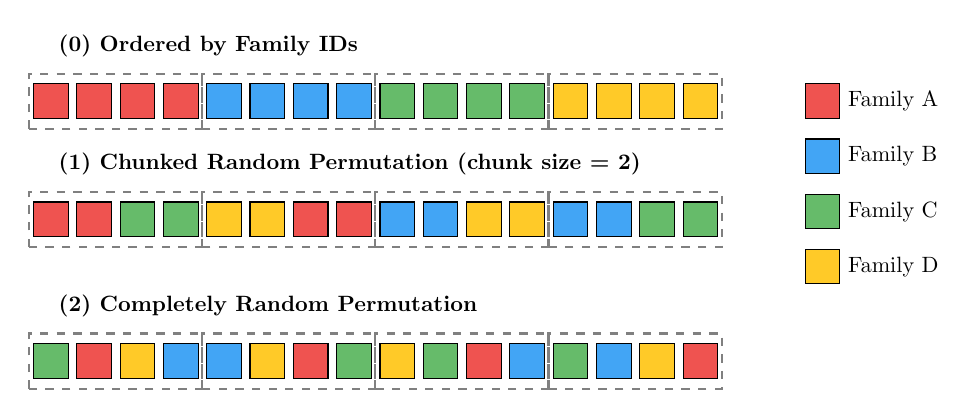
\begin{tikzpicture}[scale=1, every node/.style={scale=0.8}]
    \definecolor{famA}{RGB}{239,83,80}  
    \definecolor{famB}{RGB}{66,165,245}  
    \definecolor{famC}{RGB}{102,187,106} 
    \definecolor{famD}{RGB}{255,202,40} 
    \tikzstyle{req}=[rectangle, minimum width=0.55cm, minimum height=0.55cm, draw=black]
    \node[anchor=west] at (0,2.5) {\textbf{(0) Ordered by Family IDs}};
    \foreach \i/\col in {
        0/famA,1/famA,2/famA,3/famA,
        4/famB,5/famB,6/famB,7/famB,
        8/famC,9/famC,10/famC,11/famC,
        12/famD,13/famD,14/famD,15/famD}
        \node[req, fill=\col] at (\i*0.55,1.8) {};
    \foreach \x in {0.27,2.47,4.67,6.87}
        \draw[dashed, gray, thick] (\x-0.55,1.45) rectangle (\x+1.65,2.15);
    \node[anchor=west] at (0,1.0) {\textbf{(1) Chunked Random Permutation (chunk size = 2)}};
    \foreach \i/\col in {
        0/famA,1/famA,
        2/famC,3/famC,
        4/famD,5/famD,
        6/famA,7/famA,
        8/famB,9/famB,
        10/famD,11/famD,
        12/famB,13/famB,
        14/famC,15/famC}
        \node[req, fill=\col] at (\i*0.55,0.3) {};
    \foreach \x in {0.27,2.47,4.67,6.87}
        \draw[dashed, gray, thick] (\x-0.55,-0.05) rectangle (\x+1.65,0.65);
    \node[anchor=west] at (0,-0.8) {\textbf{(2) Completely Random Permutation}};
    \foreach \i/\col in {
        0/famC,1/famA,2/famD,3/famB,
        4/famB,5/famD,6/famA,7/famC,
        8/famD,9/famC,10/famA,11/famB,
        12/famC,13/famB,14/famD,15/famA}
        \node[req, fill=\col] at (\i*0.55,-1.5) {};
    \foreach \x in {0.27,2.47,4.67,6.87}
        \draw[dashed, gray, thick] (\x-0.55,-1.85) rectangle (\x+1.65,-1.15);
    \node[req, fill=famA, label=right:{Family A}] at (9.8,1.8) {};
    \node[req, fill=famB, label=right:{Family B}] at (9.8,1.1) {};
    \node[req, fill=famC, label=right:{Family C}] at (9.8,0.4) {};
    \node[req, fill=famD, label=right:{Family D}] at (9.8,-0.3) {};
\end{tikzpicture}}
\end{figure}
\end{frame}

\begin{frame}{Varying Multiple Parameters Together}
\begin{columns}[T, totalwidth=\textwidth]
    \begin{column}{0.6\textwidth}
        \centering
        \includegraphics[width=\textwidth]{\RESULTDIR/throughput_vs_req_batch_rand_families_10.png}
        \captionof{figure}{Throughput vs Workload by varying other parameters (10 families)}
    \end{column}
    \begin{column}{0.4\textwidth}
        \begin{itemize}
            \item Increase in batch size $\rightarrow$ higher throughput. \pause
            \item A batch nature level of 1 is roughly similar to level 2 $\rightarrow$ even a small amount of mixing leads to significant degradation. \pause
            \item A homogeneous batch of smaller size at times performs siginificantly better than a larger heterogeneous batch.
        \end{itemize}
    \end{column}
\end{columns}
\end{frame}


\begin{frame}{Varying Chunk Size while Permuting}
\begin{columns}[T, totalwidth=\textwidth]
    \begin{column}{0.5\textwidth}
        \centering
        \captionof{table}{Throughput across different $k$ levels}
        \label{tab:throughput_randomness}
        \begin{tabular}{|c|c|}
        \hline
        \textbf{$k$} & \textbf{Throughput (req/sec)} \\
        \hline
        200  & 89.35  \\
        300  & 87.49  \\
        400  & 86.50  \\
        499  & 88.19  \\
        500  & 112.66 \\
        1000 & 112.41 \\
        \hline
\end{tabular}
    \end{column}
    \begin{column}{0.5\textwidth}
        \begin{itemize}
            \item Before passing the requests to the model, we make chunks of size $k$, and permute each chunk randomly. \pause
            \item A $k$ value of 499 essentially means that in the first batch we have 499 requests of one family and 1 request of another family\pause
            \item However the throughput is much lower than a $k$ value of 500. \pause
            \item Even one request of a different family will cause L2 cache thrashing.
        \end{itemize}
    \end{column}
\end{columns}
\end{frame}

\begin{frame}{DRAM Bandwidth Utilization - for Multiple Families}
    \centering
\includegraphics[width=0.8\textwidth]{\RESULTDIR/mult_fam_drama.png}
\captionof{figure}{Comparison for $k = 500$ and $k = 499$}
\begin{itemize}
    \item L2 cache hit/miss rates $\rightarrow$ difficult to capture, as there are thousands of kernels forked. \pause
    \item DRAMA - fraction of cycles where data was sent to or received from device memory.\pause
    \item Average DRAMA for $k = 500 \rightarrow 0.18$ ; Average DRAMA for $k = 499 \rightarrow 0.22$.
\end{itemize}
\end{frame}

\section{Future Steps}

\begin{frame}{Future Steps}
\begin{itemize}
    \item \textbf{Improved Scheduler:} Design a scheduler that takes into account factors such as L2 cache size, the working set size of the current batch, the number and size of the KV cache blocks being targeted, and dynamically decides whether forming smaller homogeneous batches can outperform larger, mixed ones. \pause
    \item \textbf{SM Level Optimization:} To increase the per-SM L1 cache hit rate, it is desirable to schedule requests from the same family on nearby (or the same) SMs. One possible approach is to assign each attention kernel an identifier associated derived from its family ID and preferentially schedule it on an SM already hosting requests from that family.
\end{itemize}
\end{frame}

\begin{frame}{Future Steps}
\begin{itemize}
    \item \textbf{KV Cache Offloading:} As the number of families grows, the GPU's HBM may eventually become insufficient to hold all KV Cache blocks. Design an efficient eviction policy, ideally guided by the degree of prefix sharing among the currently scheduled batches. \pause
    \item \textbf{Response Quality:} Another promising direction is to improve response quality for requests sharing a large common context. One approach is to fine-tune the model specifically for such shared contexts and compare its performance with that of a baseline model that receives the shared context as part of a system prompt.
\end{itemize}
\end{frame}


\section{}
\begin{frame}
    \Huge{\centerline{\bf Thank You}}
\end{frame}

\end{document}
